\chapter{servlet项目}

\section{整体概述}
饿了么 Servlet 版项目是采用 VUE-CLI 与 Servlet 开发的前后端分离模式项目。前端Vue用于构建用户界面,同时在浏览器中发送XMLHttpRequest请求,
后端部分则致力于提供一套完整正确的用户点餐后端程序。

\section{项目技术架构}
VUE-CLI, JDK17, MySQL, Servlet, Tomcat8.5

\section{设计}
\subsection{功能描述}
支持用户完成整套点餐流程,包括选择商家,注册登录账户,修改账户信息,完成订单支付等功能。

\subsection{业务流程图}

\begin{figure}[htbp]
    \centering
    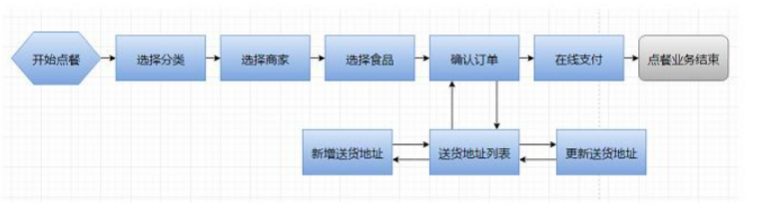
\includegraphics[width=0.8\textwidth]{servlet}
    \caption{servlet}
    \vspace{\baselineskip}
\end{figure}

\subsection{数据设计}
\subsubsection{实体类}

Business(商家)

私有变量:

商家ID:businessId(Integer)  商家名称:businessName(String)  密码:password(String)

商家地址:businessAddress(String)  商家描述信息:businessExplain(String)  起送费:starPrice(Double)

配送费:deliveryPrice(Double)  商家图片:businessImg(String)  商家类别:orderTypeId(Integer)  备注:remakrs(String))



Food(商品)

私有变量:

商品ID:foodId(Integer)  商品名:foodName(String)  商品描述信息:foodExplain(String)  价格:price(Double)

所属商家ID:businessId(Integer)  备注:remakrs(String)  商品图片:foodImg(String))



User(用户)

私有变量:

用户ID:userId(String)  用户名:userName(String)  密码:password(String)  性别:userSex(Integer)

用户头像:userImg(String)  删除标志:delTag(Integer))



Cart(购物车订单)

私有变量:

购物车订单Id:cartId(Integer)  商家ID:businessId(Integer)  商品ID:foodId(Integer)

用户ID:userId(String)  订购份数:quantity(Double))



DeliveryAddress(配送地址)

私有变量:

地址ID:daId(Integer)  联系人姓名:contactName(String)  联系人性别:contactSex(Integer)


联系人电话:contactTel  地址:address(String)  用户ID:userId(String))



Orders(订单)

私有变量:

订单Id:orderId(Integer)  用户ID:userId(String)  商家ID:businessId(Integer)


订单日期:orderDate(String)  订单金额:orderTotal(Double)  配送地址ID:daId(Integer)  订单状态:orderState(Integer))



OrderDetailet(订单明细)

私有变量:

订单明细ID:odId(Integer)  订单Id:orderId(Integer)  商品ID:foodId(Integer)  订单总量:quantity(Integer))

\subsubsection{工具类}
DBUtil(数据库连接工具):私有静态变量:DataSource(连接池工具,用来实现数据库持久连接)

CommonUtil(获取时间工具)

\subsection{数据库设计}

\begin{table}[htbp]
	\caption{商家表(点餐业务)}
	\vspace{0.5em}\wuhao
	\begin{tabularx}{\hsize}{@{\extracolsep{\fill}}c c c}
		\toprule[1.5pt]
		字段名          &  数据类型  &   说明 \\ 
		\midrule[1pt]
		businessId   & int  & 商家编号 \\
		businessName    & varchar  & 商家名称   \\
		businessAddress  & varchar & 商家地址 \\
		businessExplain     & varchar     & 商家介绍 \\
		businessImg      & mediumtext     & 商家图片 \\
		orderTypeId      & int     & 共用10种点餐分类 \\
		starPrice      & decimal     & 起送费 \\
		deliveryPrice      & decimal     & 配送费 \\
		remarks     & varchar     & 备注 \\
		\bottomrule[1.5pt]
	\end{tabularx}
	\vspace{\baselineskip}
\end{table}

\begin{table}[htbp]
	\caption{食品表(点餐业务)}
	\vspace{0.5em}\wuhao
	\begin{tabularx}{\hsize}{@{\extracolsep{\fill}}c c c}
		\toprule[1.5pt]
		字段名          &  数据类型  &   说明 \\ 
		\midrule[1pt]
		foodId      & int     & 食品编号 \\
		foodName   & varchar  & 食品名称 \\
		foodExplain    & varchar  & 食品介绍   \\
		foodImg      & mediumtext     & 食品图片 \\
		foodPrice      & decimal     & 食品价格 \\
		businessId      & int     & 所属商家编号 \\
		businessId      & varchar     & 备注 \\
		\bottomrule[1.5pt]
	\end{tabularx}
	\vspace{\baselineskip}
\end{table}

\begin{table}[htbp]
	\caption{购物车表}
	\vspace{0.5em}\wuhao
	\begin{tabularx}{\hsize}{@{\extracolsep{\fill}}c c c}
		\toprule[1.5pt]
		字段名          &  数据类型  &   说明 \\ 
		\midrule[1pt]
		cardId      & int     & 无意义编号 \\
		foodId   & int  & 食品名称 \\
		businessId    & int  & 所属商家编号   \\
		userId      & varchar     & 所属用户编号 \\
		quantity      & int     & 同一类型食品的购买数量 \\
		\bottomrule[1.5pt]
	\end{tabularx}
	\vspace{\baselineskip}
\end{table}

\begin{table}[htbp]
	\caption{送货地址表}
	\vspace{0.5em}\wuhao
	\begin{tabularx}{\hsize}{@{\extracolsep{\fill}}c c c}
		\toprule[1.5pt]
		字段名          &  数据类型  &   说明 \\ 
		\midrule[1pt]
		daId      & int     & 送货地址编号 \\
		contactName   & varchar  & 联系人姓名 \\
		contactSex    & int  & 联系人性别   \\
		contactTel   & varchar     & 联系人电话 \\
		address      & varchar     & 送货地址 \\
		userId      & varchar     & 所属用户编号 \\
		\bottomrule[1.5pt]
	\end{tabularx}
	\vspace{\baselineskip}
\end{table}

\begin{table}[htbp]
	\caption{订单表}
	\vspace{0.5em}\wuhao
	\begin{tabularx}{\hsize}{@{\extracolsep{\fill}}c c c}
		\toprule[1.5pt]
		字段名          &  数据类型  &   说明 \\ 
		\midrule[1pt]
		orderId      & int     & 订单编号 \\
		userId   & varchar  & 所属用户编号 \\
		businessId    & int  & 所属商家编号   \\
		orderDate   & varchar     & 订购日期 \\
		orderTotal      & decimal     & 订单总价 \\
		daId      & int     & 所属送货地址编号 \\
		orderState      & int     & 订单状态(0未支付,1已支付) \\
		\bottomrule[1.5pt]
	\end{tabularx}
	\vspace{\baselineskip}
\end{table}


\begin{table}[htbp]
	\caption{订单明细表}
	\vspace{0.5em}\wuhao
	\begin{tabularx}{\hsize}{@{\extracolsep{\fill}}c c c}
		\toprule[1.5pt]
		字段名          &  数据类型  &   说明 \\ 
		\midrule[1pt]
		odId      & int     & 订单明细编号 \\
		orderId   & int  & 所属订单编号 \\
		foodId    & int  & 所属食品编号   \\
		quantity   & int     & 数量 \\
		\bottomrule[1.5pt]
	\end{tabularx}
	\vspace{\baselineskip}
\end{table}

\begin{table}[htbp]
	\caption{用户表}
	\vspace{0.5em}\wuhao
	\begin{tabularx}{\hsize}{@{\extracolsep{\fill}}c c c}
		\toprule[1.5pt]
		字段名          &  数据类型  &   说明 \\ 
		\midrule[1pt]
		userId      & varchar     & 用户ID \\
		password   & varchar  & 密码 \\
		userName    & varchar  & 用户名   \\
		userSex      & int     & 性别 \\
		userImg      & mediumtext     & 用户头像 \\
		delTag      & int     & 删除标记 \\
		\bottomrule[1.5pt]
	\end{tabularx}
	\vspace{\baselineskip}
\end{table}

\subsection{程序结构}
项目三采用的MVC架构方式。

View:该模块是是负责与用户进行交互,向服务器发送用户请求,向用户发送服务器的回复。该层主要由前端部分完成。

Controller:该模块是将前前端发送的HTTP请求进行解析拆分,操作后端程序完成正确的相对应的操作。同时打包后端返回的消息成HTTP回复发送给前端。

Model:该模块是进行数据存储和数据库操作的部分。接受Controller发送的指令,对数据库进行相对应的操作,同时向Controler返回对应的消息。

\subsection{后端模块结构划分}
\subsubsection{Controller}
DispatcherServlet:处理前端发送过来的请求,将消息解析拆分发送给对应控制器的对应方法。也接收对应Controller发回的response,将它发回给前端。

Controller:接收前端控制器(DispatcherServlet)发来的请求,将其交付给Model模块处理请求,并接受Model发回的信息发回给DispatcherServlet。

\subsubsection{Model}
Service:被Controller层调用,并调用相对应的Dao层对数据库的操作方法,将相关信息发回给Controller。

Dao:对数据库进行相关操作,返回对应信息的层。

DB:后台数据库。

\subsection{结构图}

程序的结构图如图5-2所示:

\begin{figure}[htbp]
    \centering
    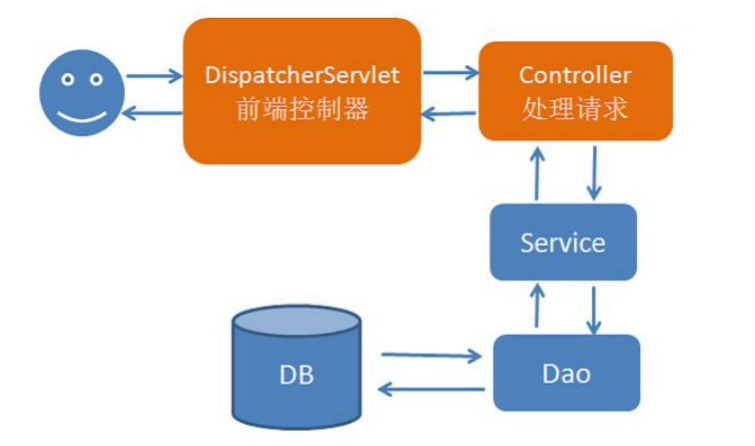
\includegraphics[width=0.8\textwidth]{MVC}
    \caption{MVC}\label{fig:MVC}
    \vspace{\baselineskip}
\end{figure}

\subsection{操作数据库接口描述}

\subsubsection{Admin}
\textbf{获取管理员对象}

getAdminByNameByPass

参数:adminName(String),password(String)

返回值:Admin

功能:传入管理员用户名和密码查找并返回对应的管理员实体。

\subsubsection{Business}
\textbf{列出相关商品类别的商家}

listBusinessByOrderTypeID

参数:orderTypeID(Integer)

返回值:List<Business>

功能:通过传入的商品类别列出此类别商家

\textbf{根据名搜索商家}

listBusinessByName

参数:businessName(String)

返回值:List<Business>

功能:通过输入字符串将商家名中含此字符串的商家列出

\textbf{根据地址搜索商家}

listBusinessByAddress

参数:businessAddress(String)

返回值:List<Business>

功能:通过输入字符串将商家字符串中含此字符串的商家列出

\textbf{获取商家}

getBusinessById

参数:businessId(Integer)

返回值:Business

功能:通过商家ID返回商家

\subsubsection{Food}
\textbf{列出商家商品}

listFoodByBusinessId

参数:businessId(Integer)

返回值:List<Food>

功能:查询数据库,列出商家ID对应商家的商品列表

\subsubsection{User}
\textbf{根据ID和密码返回账户}

getUserByIdByPass

参数:userId(String),password(String)

返回值:User

功能:根据输入的ID和密码返回对应账户

\textbf{查询账户}

getUserById

参数:userId(String)

返回值:int

功能:根据ID查询用户是否存在

\textbf{注册用户}

saveUser

参数:user(User)

返回值:int

功能:将传入的用户存入数据库

\textbf{更新用户名}

updateUserMsg

参数:userId(String),userName(String)

返回值:int

功能:修改对应ID的用户的用户名

\textbf{更新用户密码}

updateUserPassword

参数:userId(String),oldPass(String),newPass(String)

返回值:int

功能:判断密码是否正确。如果正确修改对应ID的用户的密码

\subsubsection{Cart}
\textbf{新建购物车账单}

saveCart

参数:cart(Cart)

返回值:int

功能:将传入的购物车账单存入数据库

\textbf{更新购物车}

updateCart

参数:cart(Cart)

返回值:int

功能:将与传入的购物车ID相同的购物车账单信息更新

\textbf{删除购物车账单}

removeCart

参数:cart(Cart)

返回值:int

功能:将与传入的购物车ID相同的购物车账单在数据库中删除

\textbf{列出购物车清单}

removeCart

参数:cart(Cart)

返回值:int

功能:如果存在businessId,列出对应user在此商家的购物车订单;如果不存在,列出此user所有的购物车账单

\subsubsection{DeliveryAddress}

\textbf{列出用户配送地址}

listDeliveryAddressByUserId

参数:userId(String)

返回值:List<DeliveryAddress>

功能:列出ID对应user的所有配送地址

\textbf{列出用户配送地址}

saveDeliveryAddress

参数:deliveryAddress(DeliveryAddress)

返回值:int

功能:将传入的地址存入数据库

\textbf{列出用户配送地址}

updateDeliveryAddress

参数:deliveryAddress(DeliveryAddress)

返回值:int

功能:将数据库中与传入参数daId相同的配送地址信息更新


\textbf{列出用户配送地址}

updateDeliveryAddress

参数:removeDeliveryAddress(DeliveryAddress)

返回值:int

功能:将数据库中与传入参数daId相同的配送地址删除

\textbf{根据地址ID查询地址}

getDeliveryAddressById

参数:daId(Integer)

返回值:DeliveryAddress

功能:将数据库中查询传对应daId的地址

\subsubsection{Orders}

\textbf{新建订单}

saveOrders

参数:orders(Orders)

返回值:int

功能:向数据库中存入传入的订单

\textbf{查询订单}

getOrdersById

参数:orderId(Integer)

返回值:Orders

功能:查询出与传入orderId相等的订单

\textbf{查询订单}

listOrdersByUserId

参数:userId(String)

返回值:List<Orders>

功能:列出与userId对应的用户的所有订单

\subsubsection{OrderDetailet}

\textbf{存储订单明细}

saveOrderDetailetBatch

参数:list(List<OrderDetailet>)

返回值:int

功能:将传入的订单明细组存入数据库

\textbf{存储订单明细}

listOrderDetailetByOrderId

参数:orderId(Integer)

返回值:List<OrderDetailet>

功能:列出所有数据库中与传入orderId相同的订单明细

\subsection{对外接口}
\textbf{处理http get方法}

DispatcherServlet/doGet

参数:request(HttpServletRequest) ,response(HttpServletResponse)

返回值:void

功能:处理发送的HTTP请求,将其发送给对应的Controller,让后端进行对应数据库操作,并将返回消息封装进response

\textbf{处理http Post方法}

DispatcherServlet/doPost

参数:request(HttpServletRequest) ,response(HttpServletResponse)

返回值:void

功能:处理发送的HTTP请求,将其发送给对应的Controller,让后端进行对应数据库操作,并将返回消息封装进response
\subsection{前端模块结构划分}
\begin{figure}[htbp]
    \centering
    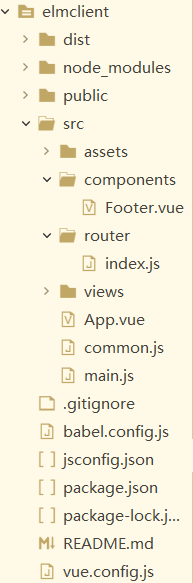
\includegraphics[width=0.4\textwidth,height=0.4\textheight]{vue1}
    \caption{前端模块结构}\label{fig:vue1}
\end{figure}
前端模块中,除了基本的项目依赖、配置文件外,主要是网页组件的制作。我们不仅需要根据不同的网页进行样式更改,还需要向服务端发送请求以获取数据资源,通过路由跳转来实现点餐过程中不同网页之间的切换。前端模块结构如图~\ref{fig:vue1}~所示

重要文件说明:
\begin{enumerate}
    \item {node\_modules文件夹}:用来存放用包管理工具下载安装的包,比如webpack、gulp、grunt这些工具。
    \item {assets文件夹}:存放网页制作所需的图片文件。
    \item {components/Footer.vue}:底部菜单组件。考虑到几乎所有页面都有底部菜单功能,为避免重复设计,我们将其单独存在Footer.vue中。在设计其他页面时,我们只需简单调用即可。
    \item {router/index.js}:路由配置文件。用来定义应用程序的路由规则,它包括了路由的基本配置信息,如路由路径、组件、重定向等,同时解决重复路由报异常的问题。
    \item {views文件夹}:用于存放不同的组件,每个组件对应一个网页。在组件中,template和style参考第四章前端项目的网页风格样式,script部分用于定义各种变量、方法,发送请求,对sessionStorage进行操作等。
    \item {App.vue}:存放共通样式,适用于所有组件。
    \item {common.js}:定义通用的方法,包括获取当前时间、向sessionStorage中增删改一个JSON对象、向localStorage中增删改一个JSON对象。
    \item {main.js}:项目的入口文件,所有的页面都会加载main.js。其作用包括:实例化Vue,设置axios的基础url部分,存储全局变量,路由守卫等。
    \item {vue.config.js}:配置文件,用于配置前端端口号、部署应用包时的基本 URL、API 请求代理等。
\end{enumerate}

\section{测试}
在本项目中,我们先对点餐的正常流程进行了测试。首先,用户可以点击首页的推荐商家列表直接选择商家,也可以在搜索框搜索商家,或通过商家分类进入符合条件的商家列表,并在商家列表中选择心仪的商家。如图~\ref{fig:order1}~和~\ref{fig:businessList}~所示.
\begin{figure}[htbp]
    \centering
    \begin{minipage}{0.4\textwidth}
        \centering
        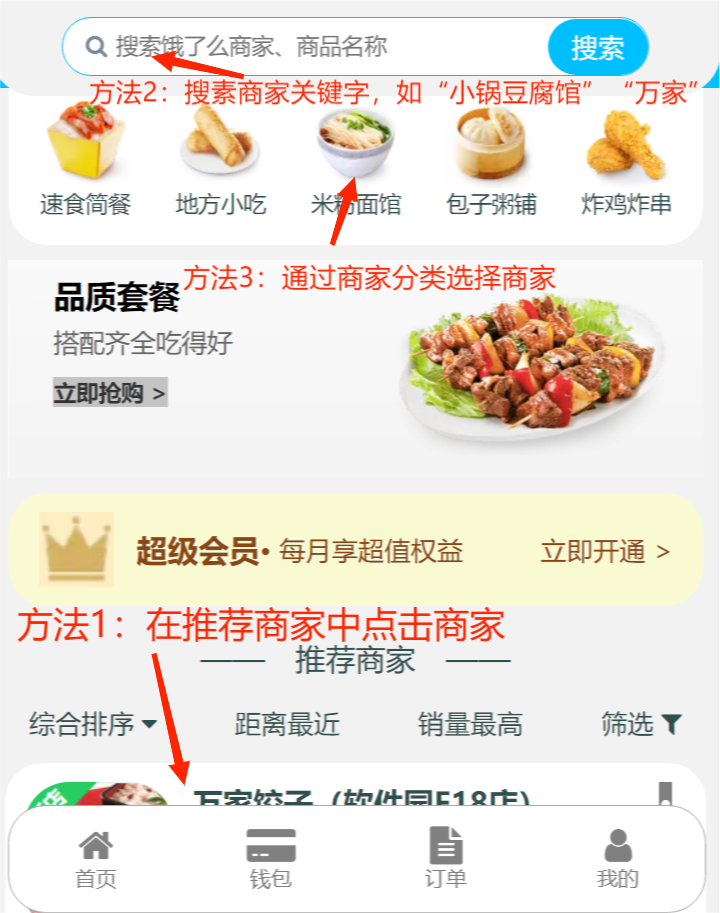
\includegraphics[width=\textwidth,height=0.3\textheight]{order1}
        \caption{选择商家的三种方法}\label{fig:order1}
    \end{minipage}
    \begin{minipage}{0.4\textwidth}
        \centering
        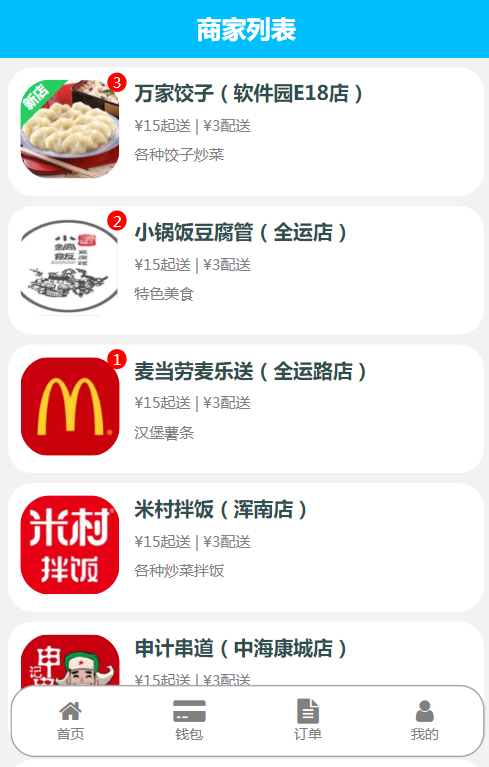
\includegraphics[width=\textwidth,height=0.3\textheight]{businessList}
        \caption{进入商家列表}\label{fig:businessList}
    \end{minipage}
    \vspace{\baselineskip}
\end{figure}

其次,进入商家后,用户可以在商家信息中进行点餐,点击“+”增加数量,点击“-”减少数量。最后点击“去结算”,此时,若用户未登录,则页面跳转至登录页面,用户可进行登录或注册操作。登陆成功后,页面重新返回,再次点击“去结算”,跳转至确认订单页面。如图~\ref{fig:order3}所示。
\begin{figure}[htbp]
    \centering
    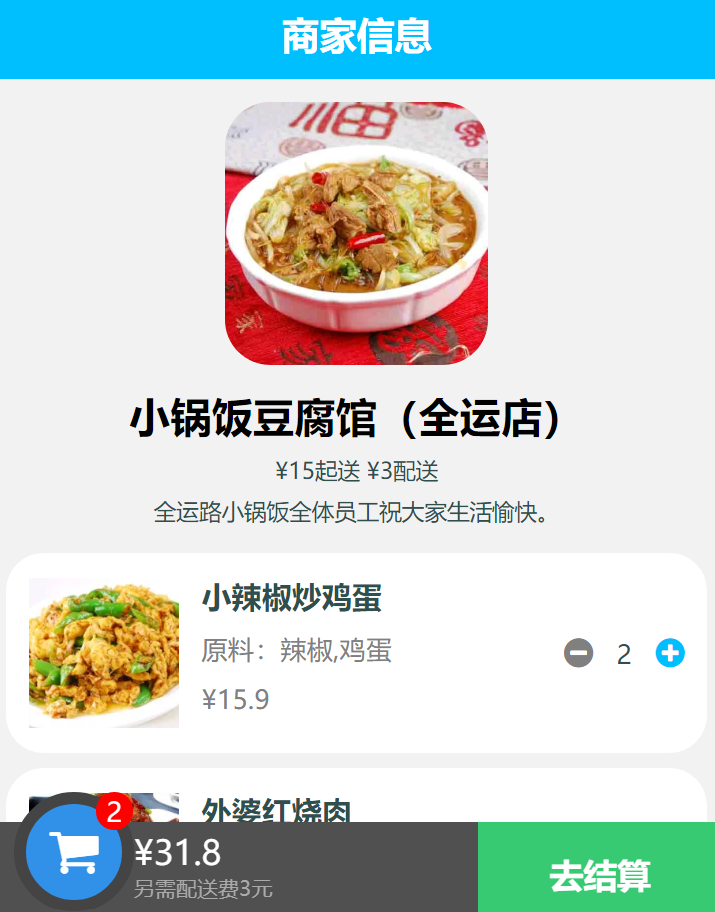
\includegraphics[width=0.4\textwidth,height=0.3\textheight]{order3}
    \caption{进入商家信息并点餐}\label{fig:order3}
\end{figure}

在确认订单页面,点击配送地址部分,可跳转至地址管理页面,对地址进行修改、删除或添加。然后点击去支付,进入支付页面。如图~\ref{fig:order5}~和~\ref{fig:userAddress}~所示.
\begin{figure}[htbp]
    \centering
    \begin{minipage}{0.4\textwidth}
        \centering
        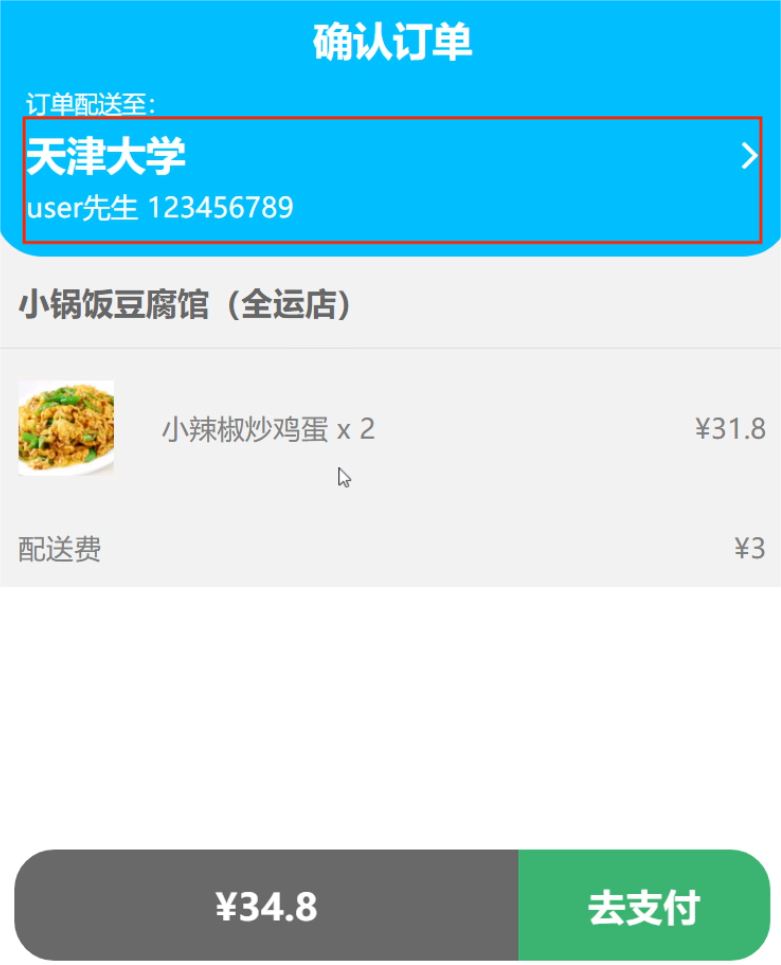
\includegraphics[width=\textwidth]{order5}
        \caption{确认订单页面}\label{fig:order5}
    \end{minipage}
    \begin{minipage}{0.4\textwidth}
        \centering
        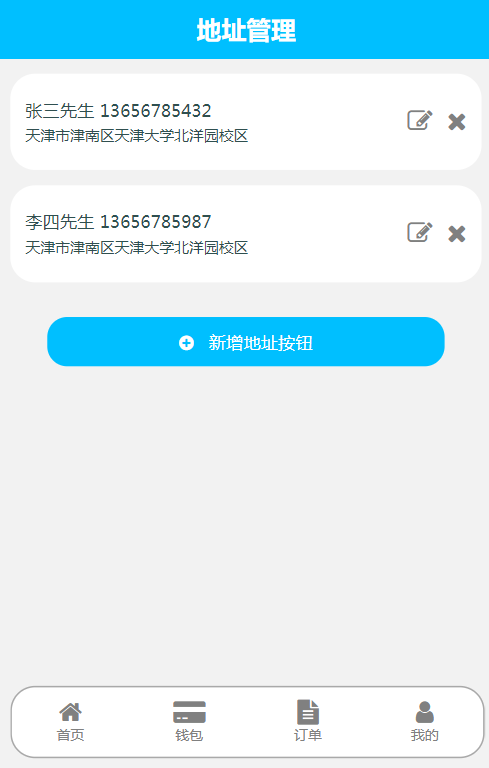
\includegraphics[width=\textwidth,height=0.3\textheight]{userAddress}
        \caption{地址管理页面}\label{fig:userAddress}
    \end{minipage}
    \vspace{\baselineskip}
\end{figure}

最后,在支付页面点击下拉按钮查看订单详情,并选择支付方式,点击“确认支付”,跳转至支付成功页面,点击“回到首页”返回首页。如图~\ref{fig:orderhidden}~和~\ref{fig:paymentDone1}~所示.

\begin{figure}[htbp]
    \centering
    \begin{minipage}{0.4\textwidth}
        \centering
        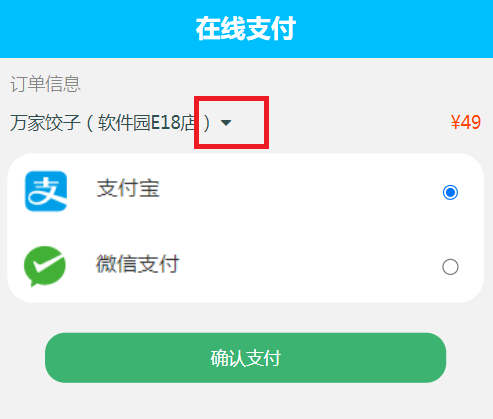
\includegraphics[width=\textwidth]{orderhidden}
        \caption{支付页面}\label{fig:orderhidden}
    \end{minipage}
    \begin{minipage}{0.4\textwidth}
        \centering
        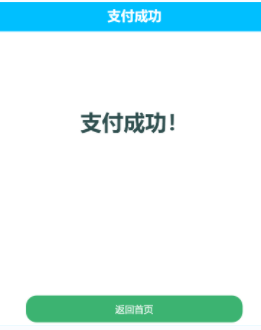
\includegraphics[width=\textwidth,height=0.25\textheight]{paymentDone1}
        \caption{支付成功页面}\label{fig:paymentDone1}
    \end{minipage}
\end{figure}
此外,针对几个重要的页面,我们对其进行了进一步的测试:
\begin{enumerate}
    \item{注册}:
    \begin{itemize}
        \item{输入数据}:手机号码:12345678911;密码:123;确认密码:111;用户名称:user;性别:女;
        \item {预期结果}:两次输入的密码不一致!
        \item {实际结果}:如图~\ref{fig:conflictingPass}~所示.
              \begin{figure}[htbp]
                  \centering
                  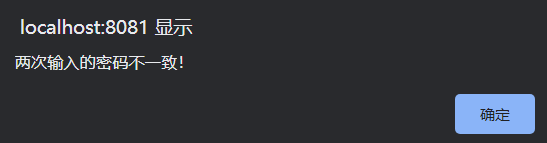
\includegraphics[width=0.6\textwidth]{conflictingPass}
                  \caption{注册密码不一致图}\label{fig:conflictingPass}
              \end{figure}
              ~\\
              \item{输入数据}:手机号码:12345678911;密码:123;确认密码:123;用户名称:user;性别:女;
        \item {预期结果}:注册成功并跳转至登录页面
        \item {实际结果}:注册成功并跳转至登录页面.如图~\ref{fig:login1}~所示.
              \begin{figure}[htbp]
                  \centering
                  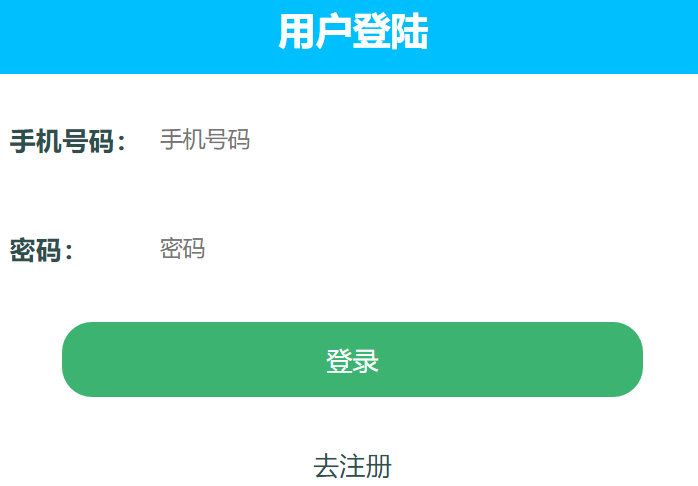
\includegraphics[width=0.4\textwidth,height=0.13\textheight]{login1}
                  \caption{注册成功返回登录的图}\label{fig:login1}
              \end{figure}
              ~\\
              \item{预置条件}:手机号12345678911已注册
              \item{输入数据}:手机号码:12345678911;密码:123;确认密码:123;用户名称:user;性别:女;
        \item {预期结果}:此手机号码已存在!
        \item {实际结果}:如图~\ref{fig:existingTel}~所示.
              \begin{figure}[htbp]
                  \centering
                  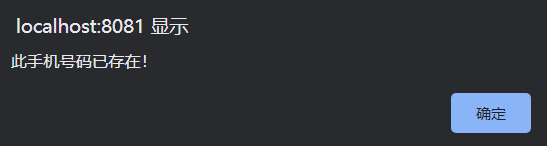
\includegraphics[width=0.5\textwidth,height=0.08\textheight]{existingTel}
                  \caption{重复注册图}\label{fig:existingTel}
              \end{figure}
    \end{itemize}
    \item {登录}:
          \begin{itemize}
              \item{预置条件}:手机号12345678911已注册
              \item{输入数据}:手机号码:12345678911;密码:123;
              \item{预期结果}:若上一个页面为注册页面,则返回首页,否则返回登录前的页面
              \item{实际结果}:当上一个页面为注册页面时,登录后仍返回注册页面
              \item{解决办法}:前端页面跳转至login前,记录来时的路由,并判断是否为register,若是,则登录成功后跳转至首页,否则跳转至来时的路由。如图~\ref{fig:beforeRouter}~和~\ref{fig:isRegister}~所示.
              \begin{figure}[htbp]
                  \centering
                  \begin{minipage}{0.4\textwidth}
                      \centering
                      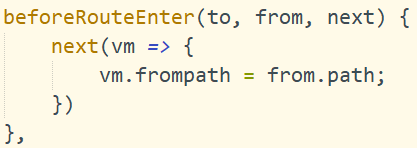
\includegraphics[width=\textwidth]{beforeRouter}
                      \caption{记录来时的路由}\label{fig:beforeRouter}
                  \end{minipage}
                  \begin{minipage}{0.4\textwidth}
                      \centering
                      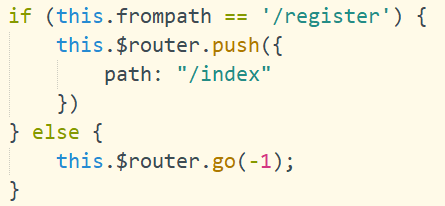
\includegraphics[width=\textwidth,height=0.095\textheight]{isRegister}
                      \caption{判断来时的路由}\label{fig:isRegister}
                  \end{minipage}                 
              \end{figure}
          \end{itemize}
    \item {“订单”页面}:
          \begin{itemize}
              \item{操作说明}:点击下拉按钮查看订单详情,点击“去支付”支付订单
              \item {预期结果}:可以看到点餐详情,“去支付”后跳转至支付页面
              \item {实际结果}:如图~\ref{fig:detail}~和~\ref{fig:orderhidden}~所示.
                    \begin{figure}[htbp]
                        \centering
                        \begin{minipage}{0.35\textwidth}
                            \centering
                            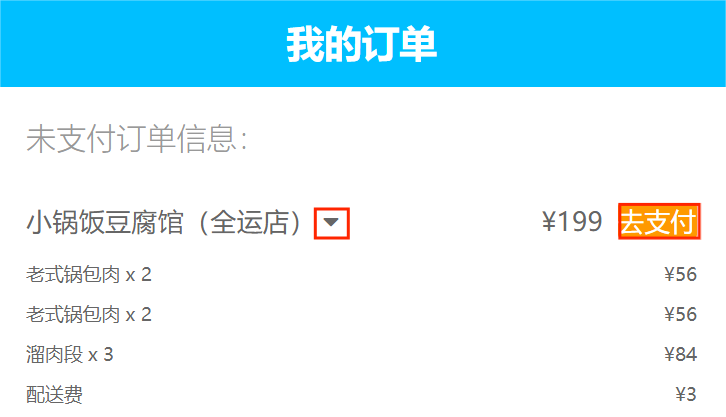
\includegraphics[width=\textwidth,height=0.1\textheight]{detail}
                            \caption{订单详情}\label{fig:detail}
                        \end{minipage}
                        \begin{minipage}{0.35\textwidth}
                            \centering
                            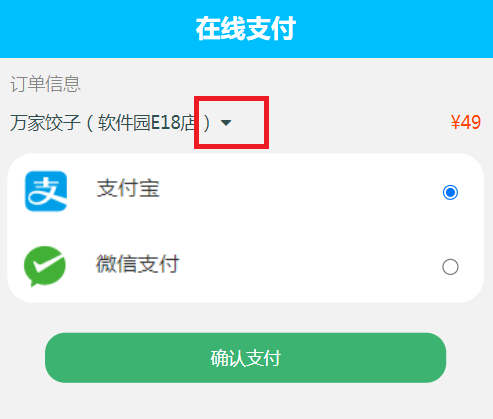
\includegraphics[width=\textwidth,height=0.1\textheight]{orderhidden}
                            \caption{去支付}\label{fig:orderhidden}
                        \end{minipage}
                        \vspace{\baselineskip}
                    \end{figure}
          \end{itemize}

    \item {“我的”页面}:
          \begin{itemize}
              \item{操作说明}:点击用户名旁的编辑按钮,更改用户名为“张三”
              \item {预期结果}:“我的”页面用户名更改为“张三”
              \item {实际结果}:数据库用户名更改成功,但“我的”页面用户名仍为原用户名
              \item {解决办法}:向sessionStorage中存储新的user对象。如图~\ref{fig:setNewName}~和~\ref{fig:updateName}~所示.
          \end{itemize}
          \begin{figure}[htbp]
            \centering
            \begin{minipage}{0.4\textwidth}
                \centering
                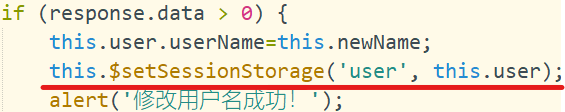
\includegraphics[width=\textwidth]{setNewName}
                \caption{SessionStorage修改}\label{fig:setNewName}
            \end{minipage}
            \begin{minipage}{0.4\textwidth}
                \centering
                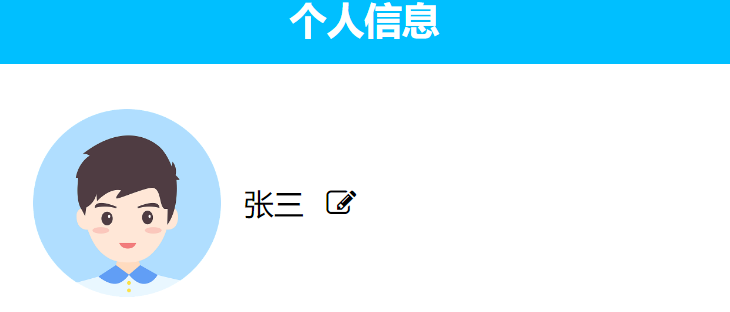
\includegraphics[width=\textwidth]{updateName}
                \caption{更改用户名成功图}\label{fig:updateName}
            \end{minipage}
        \end{figure}
          \begin{itemize}
              \item{操作说明}:点击“修改密码”,第一次在“旧密码”中输入错误密码;第二次在“旧密码”中输入正确密码。
              \item {预期结果}:第一次修改密码失败;第二次修改密码成功。
              \item {实际结果}:第一次修改密码失败;第二次修改密码成功。如图~\ref{fig:errorPass}~和~\ref{fig:correctPass}~所示.
          \end{itemize}
          \begin{figure}[htbp]
              \centering
              \begin{minipage}{0.4\textwidth}
                  \centering
                  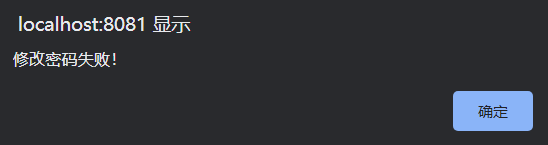
\includegraphics[width=\textwidth]{errorPass}
                  \caption{更改密码失败图}\label{fig:errorPass}
              \end{minipage}
              \begin{minipage}{0.4\textwidth}
                  \centering
                  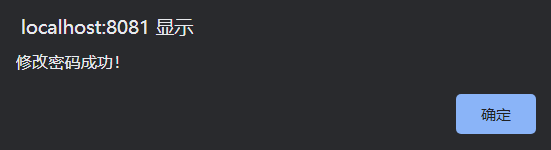
\includegraphics[width=\textwidth]{correctPass}
                  \caption{更改密码成功图}\label{fig:correctPass}
              \end{minipage}
          \end{figure}
          \begin{itemize}
              \item{操作说明}:点击“我的地址”
              \item {预期结果}:进入“地址管理”页面,可进行地址的增删改
              \item {实际结果}:完成“地址管理”页面中地址的增删改功能。如图~\ref{fig:address}~所示.
          \end{itemize}
          \begin{figure}[htbp]
              \centering
              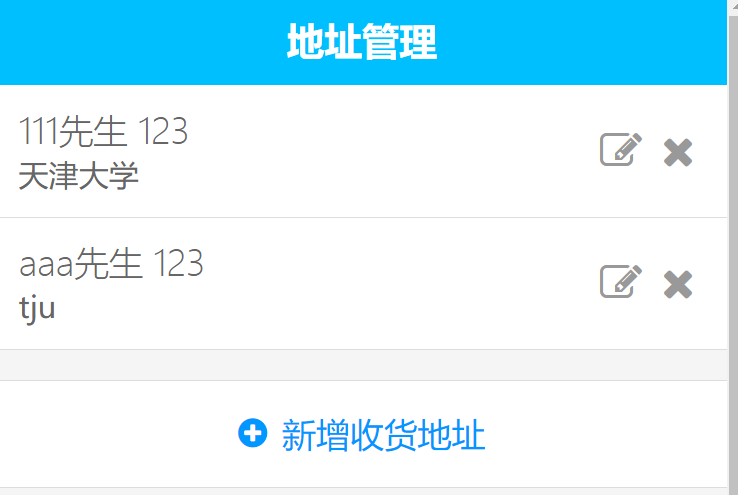
\includegraphics[width=0.4\textwidth]{address}
              \caption{地址管理}\label{fig:address}
          \end{figure}
          \begin{itemize}
              \item{操作说明}:点击“退出登录”
              \item {预期结果}:返回登录页面,用户再次访问时需登录认证
              \item {实际结果}:返回登录页面,但用户再次访问时仍保持登录状态
              \item {解决办法}:在退出登录后,前端需要从sessionStorage中移除user对象。如图~\ref{fig:withdrew}~所示.
          \end{itemize}
          \begin{figure}[htbp]
              \centering
              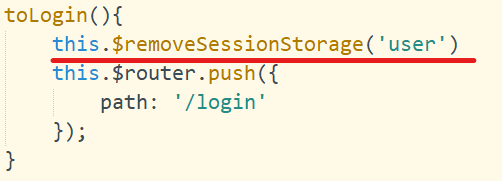
\includegraphics[width=0.4\textwidth]{withdrew}
              \caption{退出登录}\label{fig:withdrew}
          \end{figure}

\end{enumerate}

\section{部署}
\begin{itemize}
    \item{开发工具}:hbuilder、STS(spring-tool-suite)、Tomcat8.5、mysql-5.5.62-winx64
    \item {前端部署}:
          \begin{itemize}
              \item 安装 Node.js、Vue-Cli
              \item 打开hbuilder,点击文件-导入-从本地目录导入,将前端工程导入到 hbuilder 中
              \item 在cmd中,使用cd命令切换到项目路径下,使用命令npm install安装依赖, 安装成功后,在项目文件夹下出现 node\_modules 文件夹,里面是项目依赖
              \item 输入命令 npm run serve 启动项目,在浏览器中输入网址 $http://localhost:8081$,进入首页
          \end{itemize}
    \item {后端部署}:
          \begin{itemize}
              \item 安装 jdk、STS、Tomcat、MySql
              \item 在 mysql 数据库中创建数据库 elm,使用数据库脚本 elm.sql 创建数据库和初始数据
              \item 在 STS 中导入 elm 项目,并部署到 Tomcat 中
              \item 打开 com/neusoft/elm/util/dbcp.properties 修改数据库密码
              \item 在Servers上启动Tomcat
          \end{itemize}
\end{itemize}

